\documentclass[12pt]{article}

% Page setup
\usepackage{setspace}
    \doublespacing%
\usepackage{helvet}
    \renewcommand\familydefault{\sfdefault} 
\usepackage[T1]{fontenc}
\usepackage[utf8,applemac]{inputenc}
\usepackage[margin=1in, includefoot, footskip=30pt]{geometry}

% Packages
\usepackage{caption}
\usepackage{color}
\usepackage{amssymb}
\usepackage{booktabs}
\usepackage{graphicx}
\usepackage{hyperref}
\usepackage{wrapfig}
\usepackage{rotating}
\usepackage{floatpag}
    \floatpagestyle{plain}
    \renewcommand{\arraystretch}{.6}
\usepackage{amsthm}
    \newtheorem{definition}{Definition}

\newlength{\imgwidth}
\newlength{\logoheight}
\setlength{\imgwidth}{.725\paperwidth}
\setlength{\logoheight}{.125\paperheight}
\DeclareUnicodeCharacter{2010}{-}

\title{Novel methods for the analysis of NHS patient-episode data}
\author{%
    Henry Wilde\\
    \small{\textit{Supervised by:} Dr Jonathan Gillard \& Dr Vincent Knight}
}


\begin{document}
\titlepage{%
    \maketitle
    \vfill%
    \makebox[\linewidth]{%
        \includegraphics[height=\logoheight]{../img/cu_logo.png}%
        \hfill%
        
\includegraphics[height=\logoheight]{../img/cthb_logo.jpg}
    }
    \thispagestyle{empty}
    \pagebreak%
}

\tableofcontents%
\thispagestyle{empty}
\pagebreak%
\setcounter{page}{1}

In this section we will conduct a summative and exploratory analysis of the data
provided by the Cwm Taf University Health Board. The focus will be on the
distributions of, and relationships between, our non-trivial cost components
and a selection of other clinical attributes such as length of stay and number
of diagnoses. As we will see in the ensuing analysis, the bulk of this data
corresponds to short-stay and relatively low-cost spells of treatment. Following
this, we will endeavour to construct a framework for the analysis of slices
within the data which provide another dimension to our analysis through
comparison and contrast. However, before any such analysis begins, it is
important to understand the structure of data we are dealing with and how it has
been prepared.

\subsection{Data structure}\label{subsec:structure}

The data is comprised of approximately two and a half million episode-level
records for patients from across Wales that are being treated in the Prince
Charles and Royal Glamorgan hospitals. An episode is defined to be any
continuous period of care provided by the same consultant in the same place. For
instance, if a patient is admitted to a general medical ward for diagnosis and
testing, and then is referred to a specialist consultant in oncology their first
episode would end and be recorded, and a second episode of care would begin on
the oncology ward. Each of these episodes would correspond to a row in the
dataset. If the patient was then discharged, they would have completed a spell
with two episodes. In this analysis we will avoid looking at episode-level
statistics in favour of a patient's spell-level statistics. Since the
introduction of the `payment by results' system for financial flows, it has been
seen that focusing on the more granular episode statistics can lead to the
amount of resource or `activity' consumed by a hospital to treat that patient
being overestimated~\cite{BMJ2004}.

Each episode is recorded as a row of roughly 250 attributes or columns,
including:

\begin{itemize}
    \item Personal identifiers such as identification numbers, age, registered
        GP practice, as well as spell admission and discharge dates;
    \item Other clinical quantities such as the number of diagnoses and
        procedures conducted in that episode, admission and discharge methods,
        and length of stay;
    \item A number of cost components which include the costs coming from
        various departments within the hospital, ward and overhead costs, and
        the cost of administration;
    \item Diagnosis (HRG, ICD10) and procedure (OPCS4) indicators, as well as
        Charlson index scores for a selection of common diagnoses.
\end{itemize}

Of the attributes listed here, we will focus on the cost components and other
clinical variables, paying particular attention to those attributes which are
considered to be linked to overall contribution to the cost of care. Other than
the cost components themselves, those attributes are: true length of stay,
maximum number of diagnoses and total number of procedures in a spell, and the
number of spells associated with any given patient.

\subsection{Cleaning the data}\label{subsec:formatting}

As with many \-- if not all \-- machine learning and knowledge discovery
applications, a substantial amount of preprocessing and formatting was required
to make the data consistent and suitable for our purposes. This process included
the removal of some superfluous columns which added no real information to the
dataset, and a number of rows that had been corrupted by some external storage
software during data collection. In addition to this, we reformatted some
columns whose entries were intended to be used as datetime objects later on.

\graphicspath{{./img/overview/}}
\section{An overview of the data}\label{sec:overview}

As was discussed in Section~\ref{subsec:structure}, the majority of the
attributes in the dataset will not be considered at this stage of the analysis,
allowing the focus to be on how the cost of care is distributed and seen in the
data. This subset will frequently be referred to as the set of `key attributes'.
The exclusion of the other attributes does not, however, imply that they
are not of interest or that they are in any way unimportant.

The chosen attributes provide a base for understanding how the costs and
resources consumed by a patient in a spell are built up: cost components give
direct evidence as to which departments and types of procedures are being
utilised; the length of stay can give an indication of the nature of the spell
and any default costs that are incurred; and considering the maximum and total
number of diagnoses and procedures (respectively) in a spell allow for some
insight into the severity or complexity of a patient's spell in hospital.

\subsection{Distributions and summative
statistics}\label{subsec:distributions_statistics}

When looking at the distributions of the key attributes on the whole dataset, it
is seen that the data is weighted towards low-cost, short-stay, and
otherwise low-impact patients. The distributions themselves have long, and often
heavy, tails. This can be seen in
Figures~\ref{fig:netcost_kde}\--\ref{fig:no_spells_bar}.

\begin{figure}[htbp]
    \centering
    \includegraphics[width=\imgwidth]{netcost_kde/main.pdf}
    \caption{Estimated probability density for the net cost of a spell, clipped
        at \pounds12,500. \textit{Maximum approx.
        \pounds369,000.}}\label{fig:netcost_kde}
\end{figure}

\begin{figure}[htbp]
    \includegraphics[width=\imgwidth]{los_bar/main.pdf}
    \caption{Bar chart for the total length of a spell, clipped at 21 days.
        \textit{Maximum 705 days.}}\label{fig:los_bar}
\end{figure}

\begin{figure}[htbp]
    \centering
    \includegraphics[width=\imgwidth]{no_diag_bar/main.pdf}
    \caption{Bar chart for the number of diagnoses in an
        episode.}\label{fig:no_diag_bar}
\end{figure}

\begin{figure}[htbp]
    \centering
    \includegraphics[width=\imgwidth]{no_proc_bar/main.pdf}
    \caption{Bar chart for the number of procedures in an
        episode.}\label{fig:no_proc_bar}
\end{figure}

As can clearly be seen, the dataset has some significant skew. In particular,
when inspecting Figures~\ref{fig:los_bar}~\&~\ref{fig:no_spells_bar},
the majority of lengths of stay and total numbers of stays for patients are
minimal, i.e.\ of all the spells provided under the care of the health board,
the majority of them are daycases and the patients they deal with are one-off
treatments.

\begin{figure}[htbp]
    \centering
    \includegraphics[width=\imgwidth]{no_spells_bar/main.pdf}
    \caption{Bar chart for the number of spells associated with a
        patient.}\label{fig:no_spells_bar}
\end{figure}

\begin{figure}[htbp]
    \centering
    \includegraphics[width=\imgwidth]{age_bar/main.pdf}
    \caption{Bar chart for the age of patients with two-year
        bins.}\label{fig:age_bar}
\end{figure}

However, this does not imply that these spells all come cheap. When we look at
the distribution of the net cost of a spell (Figure~\ref{fig:netcost_kde}) we
see that although there is a distinct peak around a relatively low net cost,
this value has probability \(7.5\times10^{-4}\ (2 sf.)\). That is, the most
likely net cost of treating a patient in this dataset occurs less than one tenth
of a percent of the time, and the overwhelming majority of recorded net costs
are spread over a massive range. While tests do exist for verifying if our
empirical data is truly heavy-tailed~\cite{Bryson1974}, it is clear our net
costs (at least) are distributed in such a way. Further results on the
distributions of our net and component costs can be seen in
Table~\ref{tab:summative}.

\begin{table}[htbp!]
    \resizebox{\textwidth}{!}{%
        \begin{tabular}{lrrrrrrrrrr}
\toprule
{} &       COST &       CRIT &      DRUG &      EMER &      ENDO &       HCD &       IMG &   IMG\_OTH &        MED &       NCI \\
\midrule
mean &    1834.93 &     -92.08 &     75.40 &      1.24 &     21.19 &     20.91 &     32.70 &     20.57 &     347.12 &    -30.92 \\
std  &    3771.16 &    1332.61 &    315.17 &     29.13 &     92.76 &    210.98 &    143.67 &    118.26 &     739.73 &     85.80 \\
min  &       4.50 & -250000.61 &     -0.57 &      0.00 &      0.00 &      0.00 &      0.00 &      0.00 &       0.00 & -12960.21 \\
25\%  &     347.67 &       0.00 &      7.18 &      0.00 &      0.00 &      0.00 &      0.00 &      0.00 &      44.45 &    -29.75 \\
50\%  &     749.49 &       0.00 &     20.00 &      0.00 &      0.00 &      0.23 &      0.08 &      0.00 &     130.67 &    -11.64 \\
75\%  &    1886.38 &       0.00 &     59.88 &      0.00 &      0.00 &      4.83 &     10.93 &      0.31 &     375.32 &     -3.02 \\
max  &  369168.93 &       0.00 &  63430.52 &  33347.89 &  11855.95 &  94411.85 &  46708.66 &  46708.66 &  116449.90 &      0.00 \\
\bottomrule
\end{tabular}

    }
    \resizebox{\textwidth}{!}{%
        \begin{tabular}{lrrrrrrrrrr}
\toprule
{} &       NID &    NetCost &     OCLST &       OPTH &      OTH &  OTH\_OTH &      OUTP &        OVH &      PATH &  PATH\_OTH \\
\midrule
mean &     94.83 &    1742.85 &     13.30 &     160.11 &     1.37 &     0.97 &      0.57 &     354.82 &     36.20 &     23.29 \\
std  &    248.16 &    3185.31 &     58.74 &     486.24 &    11.67 &    10.15 &     26.79 &     734.05 &    135.47 &    122.71 \\
min  &      0.00 &       4.50 &      0.00 &       0.00 &     0.00 &     0.00 &      0.00 &       0.00 &      0.00 &      0.00 \\
25\%  &     14.99 &     347.32 &      0.00 &       0.00 &     0.00 &     0.00 &      0.00 &      84.86 &      0.00 &      0.00 \\
50\%  &     32.25 &     747.13 &      0.77 &       0.00 &     0.00 &     0.00 &      0.00 &     139.47 &      4.63 &      0.00 \\
75\%  &     83.36 &    1862.51 &      5.43 &       0.04 &     0.00 &     0.00 &      0.00 &     320.93 &     31.89 &     13.76 \\
max  &  84374.21 &  369168.93 &  12358.37 &  111396.20 &  1248.83 &  1248.83 &  10632.15 &  106428.61 &  70008.12 &  70008.12 \\
\bottomrule
\end{tabular}

    }
    \resizebox{\textwidth}{!}{%
        \begin{tabular}{lrrrrrrrrrr}
\toprule
{} &  PATH\_OTH &      PHAR &  PROC\_NO &      PROS &   RADTH &     SECC &       SPS &       THER &  TRUE\_LOS &       WARD \\
\midrule
mean &     23.29 &     30.47 &     1.90 &     40.71 &    0.65 &     0.87 &     11.81 &      28.62 &      2.90 &     497.07 \\
std  &    122.71 &     86.70 &     2.21 &    343.57 &    8.01 &    27.43 &    149.46 &     181.58 &      9.21 &    1236.63 \\
min  &      0.00 &      0.00 &     0.00 &      0.00 &    0.00 &     0.00 &      0.00 &       0.00 &      0.00 &       0.00 \\
25\%  &      0.00 &      2.26 &     0.00 &      0.00 &    0.00 &     0.00 &      0.00 &       0.09 &      0.00 &      10.33 \\
50\%  &      0.00 &      7.24 &     1.00 &      0.00 &    0.00 &     0.00 &      0.00 &       0.63 &      0.00 &     142.01 \\
75\%  &     13.76 &     26.21 &     3.00 &      0.00 &    0.00 &     0.00 &      0.00 &      10.49 &      2.00 &     463.04 \\
max  &  70008.12 &  25087.73 &    70.00 &  33930.70 &  227.64 &  2177.74 &  68029.58 &  125249.49 &   3659.00 &  203854.11 \\
\bottomrule
\end{tabular}

    }
    \caption{Summative spell-level statistics for each of our non-trivial cost
    components and our selected clinical variables.}\label{tab:summative}
\end{table}

There are methods available to attempt to overcome this skewedness, including
the scaling and transformation of our numerical attributes, but they are not
necessary for the purposes of a summative analysis, though this process could
improve the performance of several algorithms on the dataset since it is of
mixed type. Moreover, the presence of this skewedness in some attributes is not
to say that all the attributes are so harshly skewed; for instance,
Figure~\ref{fig:age_bar} shows the clear peaks and troughs in the distribution
of the ages of our patients. It is clear that the distribution of ages does not
have a bell-shaped curve and should likely not be modelled as normally
distributed \-- or otherwise `bell-shaped', for that matter.

\subsection{Pairwise correlation}\label{subsec:corr}

Figure~\ref{fig:corr_heatmap} shows the Pearson correlation coefficient of all
pairs in our subset of selected attributes (not including age or number of
spells) in the form of a heatmap with a colour bar is located to the right of
it. Using a visual aid such as this makes gaining insight from our array of
numbers, and thus the relationships between our variables, much easier than
studying a table or matrix directly. It should also be noted that these
attributes are considered at the spell level again.

\begin{figure}[htbp]
    \makebox[\textwidth]{%
        \centering
        \includegraphics[height=.5\paperheight]{corr_heatmap/main.pdf}
    }
    \caption{A heatmap of the pairwise correlation coefficients for our cost
    components, and our other clinical attributes.}\label{fig:corr_heatmap}
\end{figure}

Upon inspection of Figure~\ref{fig:corr_heatmap}, we see that there are several
cost components, such as secondary commisioning costs (SECC) and emergency care
(EMER), that have no significant linear correlation with any of the other
attributes. While there seems to be an abundance of non-correlation across the
heatmap, there are clear correlations between many of our attributes; some of
these are easier to realise than others. For instance, ignoring the main
diagonal, the largest value is that between total costs (COST) and net costs at
\(0.94\). This indicates almost total positive linear correlation between these
two variables, and that makes sense given that our net cost is just the total
cost corrected for a number of reimbursable costs like critical care (CRIT)
and non-contracted income (NCI) which are entered as negative values in the
dataset \-- hence the distinctly negative correlation coefficients they have
with the other variables. Typically, these costs are small (see
Table~\ref{tab:summative}) so we would expect a strong correlation between costs
and net costs.

Another example is the strong correlation amongst the length of stay
(TRUE\_LOS), and ward and overhead costs (WARD and OVH respectively). We can
justify these anecdotally: the longer a patient spends in hospital, the more
time they are likely to spend on a ward and incurring associated overheads like
administration work and cleaning costs. It should also be clear that these
attributes all share a strong linear correlation with the net cost of a spell.
This implies that these costs and the length of stay are good indicators of the
net cost of treating someone, and may suggest that the cost components make up a
substantial and relatively consistent part of the net cost.

\subsection{Measuring variation and importance in our cost components}

The purpose of this entire work is to understand the factors leading to
variations in the cost of treating someone in hospital so it is fitting to look
at the constituent parts of our net cost: the cost components. In this section
we will make use of a dimensionless measure of variation for, and the mean
contribution to the net cost of, each cost component during a spell. Using these
pairs of quantities, we can compare the components against one another in an
rudimentary way.

During a preliminary analysis of our cost components, it was found that our
conclusions on the variations in each component were misled owing to the fact we
were measuring variation using the unbiased sample variance. While this quantity
is a perfectly valid unbiased estimator for the population variance, it is
entirely dependent on the scale of the attribute being considered. This
dependency is evident in Table~\ref{tab:summative}. In place of this measure we
use the coefficient of variation which is the ratio between the standard
deviation and mean, and so is scale invariant.

\begin{definition}
    Consider a population with mean \(\mu\) and standard deviation \(\sigma\).
    Then the \emph{coefficient of variation}, denoted by \(C_v\), is defined to
    be:

    \[
        C_{v} := \frac{\sigma}{\mu}
    \]

    If only a sample of the data from a population is available then the
    coefficient of variation can be estimated using the sample standard
    deviation and the sample mean analogously.
\end{definition}

In Figure~\ref{fig:cost_variation}, the coefficient of variation for each of our
cost components is shown as a bar in a bar chart. The components have been
ranked in descending order of their variations and it clear that there are a
number of strongly variant attributes. Taking secondary commisioning costs
(SECC) again, we see that its standard deviation is over thirty times the size
of its mean. This alone could explain why there seemed to be no linear
correlation with the other variables in Figure~\ref{fig:corr_heatmap} since the
values for these costs are so wildly varied. At the other end of the scale we
see that our ward and overhead costs are amongst the attributes with the
smallest variation, implying that they are consistent as was supposed in
Section~\ref{subsec:corr}. Despite this, we can conclude that these attributes
are quite highly varied when considering the entire dataset since the majority
of coefficients of variation found have size far greater than one.

\begin{figure}[h]
    \centering
    \includegraphics[width=\imgwidth]{cost_variation/main.pdf}
    \caption{Bar chart showing the coefficient of variation \(C_{v}\) of each
        cost component, and the net and total costs, in descending
        order.}\label{fig:cost_variation}
\end{figure}

At this point, knowing which of the cost components are the most highly varied
is not enough. To determine the relative importance of these findings, the
contribution of each cost component to the net cost of a spell must be
considered. After all, we only care for the components that make a significant
impact. We calculate these quantities by taking each cost component in turn,
dividing it by its corresponding net cost and taking the mean over all of these
values. We refer to this mean as the average contribution (or proportion) to the
net cost, although it is more accurately an average of the ratios between each
component and the net cost.

\begin{figure}[h]
    \centering
    \includegraphics[width=\imgwidth]{cost_contribution/main.pdf}
    \caption{Bar chart showing the average contribution of each cost component
        to the net cost of a spell, in descending
        order.}\label{fig:cost_contribution}
\end{figure}

By inspecting Figure~\ref{fig:cost_contribution}, it is seen that, on average,
ward and overhead costs are the two largest contributors to the net cost of a
spell. This is then followed by medical costs (MED) before the average
contribution drops down to roughly \(5\%\) and below for the various
department-specific cost components. Then for our most varied components in
Figure~\ref{fig:cost_variation}, we see their average contribution to net cost
is effectively negligible in comparison to the majority of our other components.

\begin{figure}[h]
    \centering
    \includegraphics[width=\textwidth]{cost_bubble_plot/main.pdf}
    \caption{A bubble plot showing the average contribution to the net cost of a
    spell along the vertical, and the coefficient of variation for that
    component as the size of its marker.}\label{fig:cost_bubble_plot}
\end{figure}

So, we can conclude that these components are not especially important. But what
about the others? The midriff of each of these plots contain many of the same
components. In order to aid understanding and interpretability of how these two
quantities relate to one another we make use of a bubble plot. Since each of the
plots are two-dimensional and can share the same horizontal axis, both of the
values can be visualised together by using the vertical axis and size as two
separate dimensions, as illustrated in Figure~\ref{fig:cost_bubble_plot}.

Figure~\ref{fig:cost_bubble_plot} can be interpreted either by first reading
along the vertical axis to find the components that make the most considerable
contribution to treating a patient and then investigating the relative variation
that component holds intrinsically in the dataset by looking at the size of its
outer marker. The reverse of this process is also perfectly logical since the
objective is to determine where the variation exists, and then how much of an
impact that has on the net cost. The latter is how
Figures~\ref{fig:cost_variation}~\&~\ref{fig:cost_contribution} we interpreted
above. The crux of interpreting this plot is that the further away a large
marker is from the zero line, the more important that component is considered.
However, small markers are also of interest since these components indicate that
the level of variation is relatively low \-- the reasons as to why unknown.

It is easily seen from this figure that our previous conclusions can still be
interpreted; that is, our largest contributors have some of the smallest
measures of variation while the smallest average contributors are more strongly
varied. What is of interest is the jump between these groups of cost components.
There does not seem to be any particular component in the midriff of
contributors that has huge, or indeed small, variation. As a result of this,
perhaps more investigation is needed into individual components and their
relationships with specific types of patient.

Also, the skewedness of our data could be having an adverse effect on the
representation of the last three plots, particularly those considering the
contribution to net cost. As was discussed earlier, this measure is not strictly
the contribution a component makes to the net cost since in some cases certain
components sum up to several multiples of the total net cost of the spell. This
is true in cases where critical care costs are taken as huge deductions from the
total cost of most the other components.

\subsection{Conclusions}

\textcolor{red}{%
    Overall conclusions and lead into the next chapter on diabetic patient
}

\graphicspath{{./img/diabetes/}}
\section{Taking a slice: diabetic patient analysis}\label{sec:diabetes}

The main conclusion to be taken away from the previous summative analysis is
that the dataset contains a huge amount of variation. Therefore, in order to
conduct more meaningful analysis, more homogenous subsets of the data must be
considered.

Classically, patients are categorised by age or condition~\cite{Vuik2016}. In
this section, the focus will be on the diabetic population within the dataset.
Since diabetes is recorded only as a primary or secondary condition in the
dataset and is not distinguished by type, the diabetic population is considered
to be any instance where diabetes is present.

The ensuing analysis will provide evidence that the diabetic population is
increasing in the Cwm Taf area, and that, despite this, the relative resource
consumption by diabetic patients has been stagnant over the data period. It will
also be seen that this population holds too much variation to make meaningful 
conclusions about the population on the whole. However, by considering a subset
based on a condition such as this, there is a natural opportunity to compare
the subset with its complement; by considering the differences and similarities
between these two datasets a new dimension is added to the analysis.


\subsection{Distributions}\label{subsec:diabetes_dists}

In much the same way as in Section~\ref{subsec:distributions_statistics}, taking
an overview of the key attributes provides some idea about how costs are
represented in the data.
Figures~\ref{fig:diabetes_no_spells_bar}~\--~\ref{fig:diabetes_netcost_kde} show
the same statistics as in the summative analysis though these figures have two
additional components: (a) in the case of bar charts, separate plots for overall
frequency and frequency density, and (b) a comparison with the non-diabetic
population on the same axes.

\begin{figure}[htbp]
    \centering
    \includegraphics[width=\imgwidth]{no_spells_bar/main.pdf}
    \caption{Bar chart for the number of spells associated with a patient in the
        presence of diabetes and not.}%
    \label{fig:diabetes_no_spells_bar}
\end{figure}

\begin{figure}[htbp]
    \includegraphics[width=\imgwidth]{los_bar/main.pdf}
    \caption{Bar chart for the total length of a spell in the presence of
        diabetes and not, clipped at 21 days. \textit{Maximum 705 days.}}%
    \label{fig:diabetes_los_bar}
\end{figure}

\begin{figure}[htbp]
    \centering
    \includegraphics[width=\imgwidth]{no_diag_bar/main.pdf}
    \caption{Bar chart for the maximum number of diagnoses in a spell in the
        presence of diabetes and not.}%
    \label{fig:diabetes_no_diag_bar}
\end{figure}

\begin{figure}[htbp]
    \centering
    \includegraphics[width=\imgwidth]{no_proc_bar/main.pdf}
    \caption{Bar chart for the total number of procedures in a spell in the
        presence of diabetes and not.}%
    \label{fig:diabetes_no_proc_bar}
\end{figure}

\begin{figure}[htbp]
    \centering
    \includegraphics[width=\imgwidth]{netcost_kde/main.pdf}
    \caption{Estimated probability density for the net cost of a spell in the
        presence of diabetes and not, clipped at \pounds12,500.}%
    \label{fig:diabetes_netcost_kde}
\end{figure}

\begin{figure}[htbp]
    \centering
    \includegraphics[width=\imgwidth]{age_bar/main.pdf}
    \caption{Bar chart for the age of patients in the presence of diabetes and
        not.}%
    \label{fig:diabetes_age_bar}
\end{figure}

\subsection{Pairwise correlation}\label{subsec:diabetes_correlation}

With an overview of how the key attributes are distributed in mind, as before,
it is a good idea to see how these attributes interact with one another. In
Figure~\ref{fig:diabetes_corr_heatmap}, the Pearson correlation coefficients
are shown between each of the pairs of the key attributes in the diabetic
population. Again, the attributes have been ranked in descending order according
to their summed absolute correlation coefficient (see
Definition~\ref{def:absolute_correlation}) to determine those with the highest
levels of interaction.

\begin{figure}[htbp]
    \makebox[\textwidth]{%
        \centering
        \includegraphics[height=.6\paperheight]{corr_heatmap/with_nums.pdf}
    }
    \caption{A heatmap of the pairwise correlation coefficients for the key cost
        attributes in diabetic patients. The attributes have been ordered
        according to their summed absolute correlation coefficient.}%
    \label{fig:diabetes_corr_heatmap}
\end{figure}

\begin{figure}[htbp]
    \makebox[\textwidth]{%
        \centering
        \includegraphics[height=.6\paperheight]{corr_difference/with_nums.pdf}
    }
    \caption{A heatmap of the difference in pairwise correlation coefficients
        between the diabetic and general populations. These attributes have been
        ordered according to the sum of their absolute values.}%
    \label{fig:diabetes_corr_difference}
\end{figure}


\subsection{Variation and relative importance}\label{subsec:diabetes_variation}

\begin{itemize}
    \item Variation/contribution plots \-- ordering same as above
    \item Bubble plot
    \item Conclusions
\end{itemize}

\graphicspath{{./img/clustering/}, {./img/external/}}
\section{Further work}

\begin{itemize}
    \item Clustering and review of methods
    \item External, social data
\end{itemize}


\clearpage
\inputencoding{utf8}
\bibliographystyle{plain}
\bibliography{references.bib}

\end{document}
